\documentclass{article}

\usepackage{fancyvrb}
\usepackage[a4paper, total={6in, 8in}]{geometry}
\usepackage[utf8]{inputenc}
\usepackage{amsthm}
\usepackage{amsmath, amssymb}
\usepackage{xcolor}	
\usepackage{tabu}
\usepackage{booktabs}
\usepackage{multirow}
\usepackage{indentfirst}
\usepackage{enumitem}
\usepackage{graphicx}
\theoremstyle{plain}
\newtheorem{theorem}{Theorem}[section]
\newtheorem{corollary}[theorem]{Corollary}
\newtheorem{definition}[theorem]{Definition}
\newtheorem{example}[theorem]{Example}
\graphicspath{Image}
\parskip=1.9mm
\linespread{1.1}
\setlength\parindent{24pt}


\renewcommand\qedsymbol{$\blacksquare$}
\renewcommand{\restriction}{\mathord{\upharpoonright}}

\title{\textbf{Simple Plagiarism Detection Utility using String Matching \\ ~ \\ Analysis and Design of Algorithms}}
\author{Seif Yehia Sallam ID: 900193668 \\ Salma Ahmed Aly ID: 900203182 \\ Sara Maged Nassef ID: 900202369 \\  Muhammad El-Mahdi ID:900202967 \\ ~ \\ The American University in Cairo}
\date{}

\begin{document}
\maketitle
\newpage
\section*{Introduction}
Plagiarism is presenting someone else’s thoughts, ideas, or expressions as one's own original work. In an academic setting plagiarism is considered a violation of academic integrity and a breach of journalistic ethics. It can lead to sanctions such as penalties, suspension, expulsion from school or work, substantial fines and even imprisonment in some extreme cases. Plagiarism is bad and unethical because it is a form of theft; by taking the ideas and words of others and pretending they are your own, you are stealing and benefiting from someone else's intellectual property. There are many reasons to avoid plagiarism. You have come to university to learn to know and speak your own mind, not merely to reproduce the opinions of others - at least not without attribution. You should avoid plagiarism because you aspire to produce work of the highest quality.That is why many universities require the use of a plagiarism detector for any project or paper submissions. For this reason we will be creating an algorithm to detect any plagiarism that occurs between the original source and the inputted values.
\newpage
\section*{Problem Definition}
Plagiarism detection or content similarity detection is the process of locating instances of plagiarism or copyright infringement within a work or document. The widespread use of computers and the advent of the Internet have made it easier to plagiarize the work of others. There are several ways of approaching this problem, the method we will be using for this project is string matching using four different algorithms: Brute Force using Hamming distance, Rabin-Karp, KMP, and Boyer-Moore. String matching refers to the problem of finding occurrence(s) of a pattern string within another string or body of text. When applied to the problem of plagiarism detection, documents are compared for verbatim text overlaps. In addition to plagiarism detection, string matching can be applied to text editor(s), information retrieval, image processing, computational biology, pattern recognition etc…

The algorithm takes in two vectors of strings where one is a vector of strings corresponding to the inputted sentences composed of n characters called text and a string of m characters called the pattern where m>=n.  We want to find a substring of the text that matches the pattern. More precisely, we want to find the number of occurrences of the person's text with other sources which will be the pattern. We will be setting a specific threshold and if the number of occurrences is equal to or larger than the threshold then that piece has been plagiarized. The threshold is usually 10-20% of the length of the text–that is the accepted percentage in an academic setting. 

\newpage
\section*{Methodology}
\subsection*{Brute Force Matching using Hamming Distance}
Hamming distance is the number of positions at which the corresponding symbols in compared strings are different. This is equivalent to the minimum number of substitutions required to transform one string into another. We will be using it to compare between every pair of characters–one from the text and one from the pattern, and if the number of subsequent characters is equal to the number of characters in one of the words in the string then we count it as a single occurrence. We loop over all characters in a single string for all strings in the vector. However, we will be using the Hamming distance technique alongside the brute force algorithm in that we will be using the hamming distance to loop over every character in the text through nested loops. The use of the hamming distance lowers the complexity as opposed to an algorithm that solely uses the brute force algorithm. An outline of the algorithm goes as follow:

\begin{Verbatim}
    int bruteforce(string pattern, string text){
            difference=pattern.length()-text.length();
            for(i = 0 -> difference){
                    while((j < text.length()) && (pattern[i+j] == text[j])){ /*if the
                            character from the pattern is identical to the text, increment j:
                            this is where hamming distance comes into play*/
                            J++; //this nested loop is what makes it the brute force approach
                        }
                    if(j == text.length()){
                            countocc++; //incrementing the number of occurences
                        }
                }
            return countocc;
        }
\end{Verbatim}
\newpage
\subsection*{Boyer-Morre Algorithm}

The idea of Boyer-Morre algorithm in string matching is that we create an array that holds the last occurances of each character in the pattern, and
any character that doesn't exist in the array is called a bad character.

The algorithm goes through all the text until it runs out of character.
If it ever finds a mismatch, the pattern is shifted until one of two options is done:

- The mismatch becomes a match.

- The pattern shifts past the length of the mismatched character.

\begin{Verbatim}
    const int characterSize = 256;
    void BadCharHueristic(string pattern, int badCharacters[characterSize]){
            for(i = 0 -> 256)
            badCharacters[i] = -1;
            for(i = 0 -> pattern.size())
            badCharacters[(int)(pattern[i])] = i;
        }
    int BoyerMooreAlgorithm(string text, string pattern){
            int badCharacters[characterSize];
            BadCharHueristic(pattern, badCharacters);
            int shift = 0;
            int numberOfMatches = 0;
            while(shift <= text.size() - pattern.size())
            {
                    //We start checking from back of the pattern to the beginning
                    int index = pattern.size() - 1;
                    /*
                    We keep decrementing the index until we reach
                    either a mismatch or index is now 0
                    */
                    while (index > -1 && pattern[index] == text[shiftAmount + index])
                    index--;
                    if (index == -1)
                    {
                            //then we found a match and we want to see any other matches
                            numberOfMatches += 1;
                            /* Condition to know whether we are matching
                            at the end of the text or not*/
                            if (shiftAmount + pattern.size() < text.size()){
                                    int badCharPos = badCharacters[int(text[shiftAmount + pattern.size()])];
                                    //Shift the text by the whole pattern
                                    shiftAmount += pattern.size() - badCharPos;
                                }
                            else
                            // shift it by 1 just to get out of the loops
                            shiftAmount += 1;
                        }
                    else
                    shiftAmount += std::max(1,
                    index - badCharacters[int(text[shiftAmount + index])]);
                }
            return numberOfMatches;
        }
\end{Verbatim}
\newpage
\subsection*{Rapin Karp Algortihm}
The idea of Rapin Karp algorithm was created by  Richard M. Karp and Michael O. Rabin to locate a precise matching in a text for a pattern string. One of its applications is detecting plagiarism, which is the main aim of this project. This algorithm resembles the idea of the rolling hash as it uses hashing for comparison by describing the pattern with a certain hash value and loops over the text to look for a value that matches this hash value. The hash value depends on the values of the asci code of each character then we use a prime number for a mod operation to get a stronger hash value.
This algorithm relies on 4 main steps
\begin{enumerate}
    \item Define a hash for pattern.
    \item Define a hash for the first text window.
    \item Repeat the following steps till the end of the text
          \begin{enumerate}
              \item if hash1==hash2, add the occurrences count by 1
              \item subtract the leftmost element from the window
              \item add a new character to the window to define the new hash value
          \end{enumerate}


\end{enumerate}
The algorithm is implemented in this way:-
\begin{verbatim}
    
counts RapinKarplookforpattern(const std::string& pat, const std::string&text, int prime)
{
    counts pair;
    int comparisons_count = 0;
    int occurrances_count = 0;
    int l1 = pat.length(), l2 = text.length(), i, j, patternhash = 0, texthash = 0, a = 1;
    
    for (i = 0; i < l1 - 1; i++){
        a = (a * n) mod prime;
    }
    
    if (l1 > l2)
        return {0, 0};
    
    
    for (i = 0; i < l1; i++){
        patternhash = (n * patternhash + pat[i]) mod prime;
        texthash = (n * texthash + text[i]) mod prime;
    }
    for (i = 0; i <= l2 - l1; i++){
        if (patternhash == texthash and ++comparisons_count){
            for (j = 0; j < l1; j++)
            {                
                if (text[i + j] != pat[j] and ++comparisons_count)    
                    break;
            }
            if (++comparisons_count and j == l1)
                ++occurrances_count;
        }
        if (i < (l2 - l1) and ++comparisons_count){
            texthash = (n * (texthash - text[i] * a) + text[i + l1]) mod prime;
            if (texthash < 0 and ++comparisons_count)
                texthash += prime;
        }
    }
    pair.comp = comparisons_count;
    pair.occ = occurrances_count;
    return pair;
}
\end{verbatim}

So the function returns two values, the comparisons count (for complexity calculations) and the occurrences count (to count the number of times matching occur)
\newpage
\subsection*{KMP Algortihm}
The Knuth-Morris-Pratt (KMP) algorithm is a string-matching algorithm that is theoretically one of the most efficient. One of the most fundamental operations in strings is pattern matching.
For example, suppose P is a given substring and T is a much longer string to be searched up. In that case, it is necessary to locate all substrings in string T that are the same as P. In this situation, string P is referred to as the pattern, and string T is referred to as the target. When talking about pattern matching in typical conditions, the initial step is to utilize the brute force approach to match the substring P with string T beginning from every element in T. Even though this method follows the idea, it has a massive burden and cannot be efficient. For example, if we use f (T) for the length of T, assuming f (T) =n and f (P) =m, and "length" refers to the total number of letters in a string, the number of letters matching operations required to find P from T is m*(n-m+1). Then, about the same time, Knuth, Morris, and Pratt found the KMP method, an improved string-matching algorithm that became comparatively fast and common by avoiding unnecessary letter comparisons.

KMP preprocesses pat[] and creates an auxiliary lps[] of size m (the same as the pattern size) to skip characters during matching. The abbreviation lps stands for longest proper prefix. An appropriate prefix does not enable the entire string to be used. Prefixes for "ABC" include "A," "AB," and "ABC."
"A" and "AB" are proper prefixes. The string's suffixes are "C," "BC," and "ABC." In sub-patterns, we look for lps. More specifically, we concentrate on pattern sub-strings, either prefix or suffix. For each sub-pattern pat[0..i], lps[i] stores the length of the maximum matched appropriate prefix that is also a suffix of the sub-pattern pat[0..i], where I = 0 to m-1.
We calculate values in lps[] during the preprocessing stage. To do so, we maintain track of the length of the longest prefix suffix value for the preceding index (using the len variable). We set lps[0] and len to zero. We increment len by 1 and apply the incremented value to lps[i] if pat[len] and pat[i] match. We update len to lps[len-1] if pat[i] and pat[len] do not match and len is not 0.\\

Below is how we can implement KMP algorithm:
\begin{verbatim}
void computeLPSArray(std::string pat, int M, int *lps, int &count)
{
    int len = 0;
    lps[0] = 0;
    int i = 1;
    while (i < M)
    {
        if (++count && pat[i] == pat[len])
        {
            len++;
            lps[i] = len;
            i++;
        }
        else
        {
            if (len != 0)
                len = lps[len - 1];
            else
            {
                lps[i] = 0;
                i++;
            }
        }
    }
}        
\end{verbatim}
Then, another KMP Search function uses the lps function to do it's search.

\newpage

\section*{Data Specifications}
There are two types of data in this project.

\subsubsection*{Plagiarism detection Program}

For this program we require the names of the files that represent a database for the text. i.e. the patterns, and the name of the file the represents the text that we are checking plagiarism in.

In the end the output of this program will be the Number of occurances of the plagiarized data and the plagiarism percentage.


\subsubsection*{String Comparison Performance Measurement}

The data for the comparison is generated by a random number generator that generates numbers between 65 and 97 that represent the values of the capital English letters A-Z. It generates a string of size $n$.
We also generate a pattern of size $m$ using the same random number generator.

\noindent The seed is randomally selected through time.

The data we used for the comparison range in sizes starting with 500 for the text and 2 for the pattern, up to 3000 with a step of 500.
We also change the pattern starting with size 2 and up to size 5. This is designed to study the infulence of the size of the pattern and the size of the text in affecting the performance of each algorithm.

\noindent The algorithms are tested upon these numbers.

\section*{Experimental Results}
Using the randomlly generated strings to find the number of comparisons between the four algorithms, the following table was produced

\begin{tabu} to \textwidth{|X|X|X|X|X|}
    \hline
    N \& M & Boyer Morre & Rapin Karp & BruteForce & KMP  \\
    \hline
    500/2  & 267         & 1004       & 1018       & 1000 \\
    \hline
    500/3  & 180         & 996        & 1017       & 1002 \\
    \hline
    500/4  & 139         & 996        & 1015       & 1003 \\
    \hline
    500/5  & 115         & 990        & 1013       & 1004 \\
    \hline
\end{tabu}
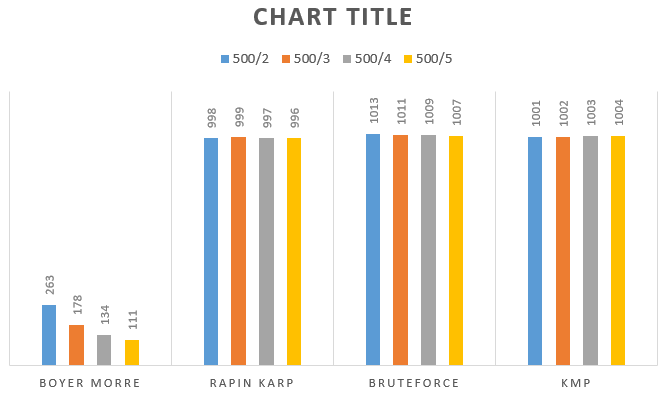
\includegraphics{Image/500.png}



\begin{tabu} to \textwidth{|X|X|X|X|X|}
    \hline
    N \& M & Boyer Morre & Rapin Karp & BruteForce & KMP  \\
    \hline
    1000/2 & 538         & 2002       & 2039       & 2001 \\
    \hline
    1000/3 & 362         & 2006       & 2037       & 2002 \\
    \hline
    1000/4 & 274         & 1998       & 2035       & 2003 \\
    \hline
    1000/5 & 228         & 1998       & 2033       & 2004 \\
    \hline
\end{tabu}
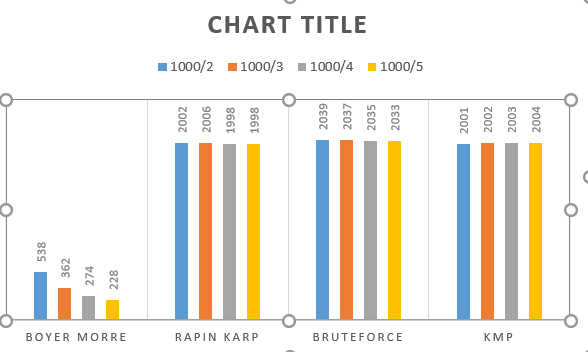
\includegraphics{Image/1000.png}




\begin{tabu} to \textwidth{|X|X|X|X|X|}
    \hline
    N \& M & Boyer Morre & Rapin Karp & BruteForce & KMP  \\
    \hline
    1500/2 & 808         & 3012       & 3061       & 2997 \\
    \hline
    1500/3 & 545         & 3016       & 3063       & 3002 \\
    \hline
    1500/4 & 418         & 3009       & 3059       & 3003 \\
    \hline
    1500/5 & 338         & 3003       & 3057       & 3004 \\
    \hline
\end{tabu}
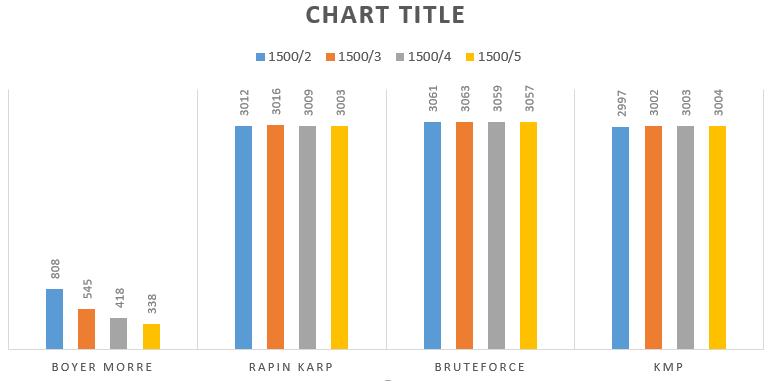
\includegraphics{Image/1500.png}



\begin{tabu} to \textwidth{|X|X|X|X|X|}
    \hline
    N \& M & Boyer Morre & Rapin Karp & BruteForce & KMP  \\
    \hline
    2000/2 & 1084        & 4024       & 4080       & 3997 \\
    \hline
    2000/3 & 727         & 4020       & 4082       & 4002 \\
    \hline
    2000/4 & 556         & 4009       & 4080       & 4003 \\
    \hline
    2000/5 & 457         & 4007       & 4078       & 4004 \\
    \hline
\end{tabu}
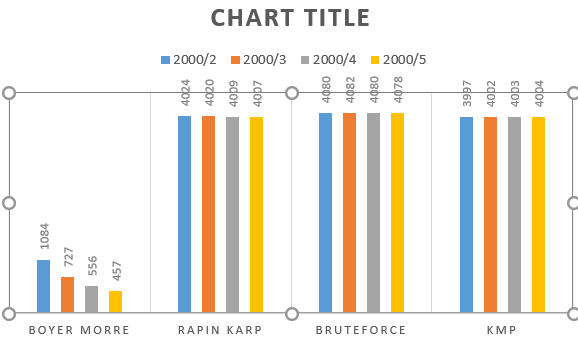
\includegraphics{Image/2000.png}





\begin{tabu} to \textwidth{|X|X|X|X|X|}
    \hline
    N \& M & Boyer Morre & Rapin Karp & BruteForce & KMP  \\
    \hline
    2500/2 & 1349        & 5026       & 5084       & 4997 \\
    \hline
    2500/3 & 899         & 5017       & 5085       & 5001 \\
    \hline
    2500/4 & 678         & 5019       & 5083       & 5002 \\
    \hline
    2500/5 & 555         & 5011       & 5081       & 5003 \\
    \hline
\end{tabu}


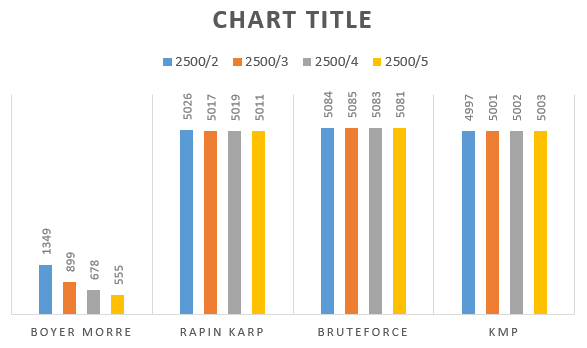
\includegraphics{Image/2500.png}











\begin{tabu} to \textwidth{|X|X|X|X|X|}
    \hline
    N \& M & Boyer Morre & Rapin Karp & BruteForce & KMP  \\
    \hline
    3000/2 & 1595        & 6048       & 6123       & 5991 \\
    \hline
    3000/3 & 1096        & 6020       & 6131       & 6002 \\
    \hline
    3000/4 & 842         & 6036       & 6129       & 6003 \\
    \hline
    3000/5 & 671         & 6023       & 6127       & 6005 \\
    \hline
\end{tabu}


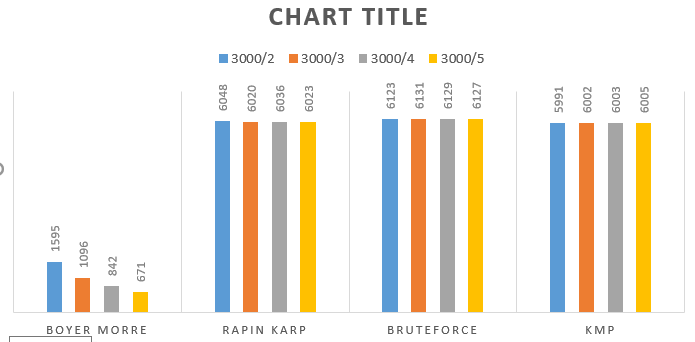
\includegraphics{Image/3000.png}


The charts provided above show the different output of the generated strings for the pattern and the text.
The charts are labeled with $n/m$ where $n$ is the size of the text, and $m$ is the size of the pattern.

These charts show how Rapin Karp, Brute force and KMP algorithms have relatively close number of comparisons so they are a bit close in terms of complexity. However, it's obvious that Boyer Morre is the most efficient algorithm as it has the lowest number of comparisons which means that it has the best complexity among these algorithms.

It's also clear how the ratio $N/M$ is proportional to the number of comparisons as it decreases as $N/M$ decreases and increases when this ratio increases.


\newpage
\section*{Analysis and Critique}
\subsection*{Boyer Morre Algorithm}
Boyer Morre algorithm consists of two procedures that are used every time the algorithm is called.

\subsubsection*{Bad Character Hueristic}

This function just initializies an array that has 256 elements and initializies them with -1 which takes $O(1)$.
It also passes through the whole pattern and sets the index in the array of which the character in the pattern represents to the current index in the pattarn, which is $O(m)$.

\noindent Total Time complexity: $O(1) + O(m) = O(m)$

\noindent Total Space complexity: $\Theta(1)$ since it is just an array of size 256

\subsubsection*{Search Algorithm}

The most inner while loop at worst case runs at the order of the size of the pattern $=> O(m)$\\
The best case for that while loop is $O(1)$

The outer most while loop at worst case runs at the order of the size of the text $=>O(n)$\\
The best case for this while loop is $\Omega(n - m)$

Space compelxity of this section of the algorithm is $O(1)$ since it doesn't require any extra space other than one integer.

Total complexity of the algorithm: $O(mn)$


Even though the complexity of this algorithm is $O(mn)$, yet it doesn't really get to that high complexity for how the algorithm works with skipping the non-promising patterns/characters it finds.

\newpage
\subsection*{Rapin Karp algorithm}
The Rapin Karp algorithm, as mentioned before, depends on the idea of the rolling hash so it loops over the text to check and compare the hash value of the pattern to each window in this text. Accordingly the time complexity of this algorithm is as follows:-
\subsubsection*{Best Case}
$T(n)= \sum_{i=0}^{l1-2} 2 + \sum_{i=0}^{l1-1} 6 + \sum_{i=0}^{l2-l1-1} 3 = 2(l1-1)+6l1+3l2-3l1=5l1+3l2-2$
$\because$ l1 is the length of pattern and l2 is the length of the text

$\therefore$ we can let $l1 = m$ and $l2=n$

$\therefore$ The best complexity is O($m+n$)

\subsubsection*{Worst Case}
$T(n)= \sum_{i=0}^{l1-2} 2 + \sum_{i=0}^{l1-1} 6 + \sum_{i=0}^{l2-l1-1} \sum_{j=0}^{l1-1}  5 = 2(l1-1)+6l1+5l1(l2-l1)= 2l1-2+6l1+5l1l2-5(l1)^2$

$\because$ l1 is the length of pattern and l2 is the length of the text

$\therefore$ we can let $l1 = m$ and $l2=n$

$\therefore$ The worst complexity is O($mn$) as mn is the most dominant part
\newpage
\subsection*{Brute Force using Hamming Distance}
Like many other brute force algorithms, string matching using Hamming distance requires two nested for looks. However, because we are using hamming distance and not just a regular brute force approach we are able to reduce the time complexity by changing the conditions for the loops. The outermost loop loops over the difference between the length of both strings being compared: the text and pattern. The innermost loop loops over the length of the pattern as long as the character in the text [i+j] is equal to that of the pattern [j]--the i+j  is for when the text is longer than the pattern. Giving the following complexities:
Take the length of the text to be n and the length of the pattern to be m:
\subsubsection*{Best Case}
Best case is when the length of the text and pattern are of equal length and not identical because if they are of equal length then the difference is 0 and it only enters the for loop once. As for the while loop, if the first character of the pattern isn't equivalent to text[i+j] then it never enters the while loop or if statement.

\noindent $T(n)= 1+ \sum_{i=0}^{n-m} 6 = 1+ 6(n-m+1)$\\
$T(n)= O(n-m+1)$\\
Which in the best case where n=m is O(1)\\
In a more regular or average case where the text is larger than the pattern the complexity stays O(n-m+1) since the difference between n and m is evident--the examples we provided in our results section. However, we can also regard finding the pattern as an average case which in this case it would have the same complexity as the worst case. The average case will depend on whether or not the pattern is found.

\subsection*{Worst Case}
The worst case is when the length of the text is much larger than the pattern and the pattern is in the text.
$T(n)= 1+ \sum_{i=0}^{n-m} \sum_{i=0}^{m} 8 $ \\
$= 1+ \sum_{i=0}^{n-m} 8(m+1)$\\
$= 1+ 8(m+1)(n-m+1)$\\
$= 1+ 8(mn-m^2+n+1)$\\
$T(n)= O(mn)$\\
\newpage
\subsection*{KMP algorithm}
The time complexity of this algorithm is as follows:-
\subsubsection*{Best Case}
$ \sum_{i=1}^{m-1} 1 = (m-1) = O(n)$,  so T(n)= O(n)

$\therefore$ The best complexity is O($n$)

\subsubsection*{Worst Case}
$ 4\sum_{i=1}^{m-1} 1 = 4(m-1) = O(n)$,  so T(n)= O(n)

$\therefore$ The worst complexity is O($n$)

\subsection*{Space complexity}
$S(n) = O(m)$ :- m is pattern length.
\newpage

\section*{Conclusion}
From the analysis section of this paper and data collected, it’s very clear that the Boyer Moore Algorithm has the lowest complexity, ergo the most efficient and best choice out of the four. It even has a better best case space complexity than the rest of the algorithms. This was eminent from the start when we looked at the guideline of the project–we were able to tell right out the gate that the Brute Force was going to have the worst complexity and Boyer Moore would have the best. Working on these algorithms taught us about the KMP and Rabin Karp approaches and when its best to use which algorithm: learning their advantages and drawbacks. In addition to calculating the complexity using the analysis techniques we learned in the course, we added a counter to each algorithm to count the number of comparisons–this is what the data was based on. It showed the extent of how much more efficient Boyer Moore is in comparison to the others. Furthermore, it highlighted how close the other three are to each other and the importance of critically evaluating every algorithm instead of taking it for face value: thinking nothing can be worse than Brute Force. While Brute Force had the highest complexity, it’s important to be aware how close KMP and Rabin Karp are to the Brute Force approach using Hamming distance and how the Hamming distance aided in lowering the complexity.

\section*{Acknowledgement}
We would like to thank our professor Amr Goneid for his clear explanation of the different aspects of the course and his Teacher Assistant Mr. Mohamed Hany for helping and guiding us throughout the semester.
\newpage
\section*{References}
Applications of string matching algorithms. (2020, September 03). Retrieved December 12, 2021, from https://www.geeksforgeeks.org/applications-of-string-matching-algorithms/

Boyer Moore algorithm for Pattern Searching. (2021, December 08). Retrieved December 12, 2021, from https://www.geeksforgeeks.org/boyer-moore-algorithm-for-pattern-searching/

Chattopadhyay, A., Jaiteh, M., \& Khim, J. (n.d.). Knuth-Morris-Pratt algorithm. Retrieved December 12, 2021, from https://brilliant.org/wiki/knuth-morris-pratt-algorithm/

Hakak, S. I., Kamsin, A., Shivakumara, P., Gilkar, G. A., Khan, W. Z., \& Imran, M. (2019). Exact string matching algorithms: Survey, issues, and future research directions. IEEE Access, 7, 69614-69637. doi:10.1109/access.2019.2914071

Hamming distance between two strings. (2021, May 19). Retrieved December 12, 2021, from https://www.geeksforgeeks.org/hamming-distance-two-strings/

Rabin-Karp algorithm. (n.d.). Retrieved December 12, 2021, from https://www.programiz.com/dsa/rabin-karp-algorithm


\newpage
\section*{Appendices}
\subsection*{Appendix A: Rabin Karp Algorithm}
\begin{verbatim}
    #include <iostream>
#include <string>
#include <cstring>
#include "../headers/RapinKarp.h"
using namespace std;
#define n 256

counts RapinKarplookforpattern(const std::string &pat, const std::string &text, int prime)
{
	counts pair;
	int comparisons_count = 0;
	int occurrances_count = 0;
	int l1 = pat.length(), l2 = text.length(), i, j, patternhash = 0, texthash = 0, a = 1;
	for (i = 0; i < l1 - 1; i++)
		a = (a * n) % prime;
	if (l1 > l2)
		return {0, 0};
	for (i = 0; i < l1; i++)
	{
		patternhash = (n * patternhash + pat[i]) % prime;
		texthash = (n * texthash + text[i]) % prime;
	}
	for (i = 0; i <= l2 - l1; i++)
	{
		if (++comparisons_count && patternhash == texthash)
		{
			for (j = 0; j < l1; j++)
			{
				if (++comparisons_count && text[i + j] != pat[j])
					break;
			}

			if (j == l1)
				++occurrances_count;
		}
		if (i < (l2 - l1))
		{
			texthash = (n * (texthash - text[i] * a) + text[i + l1]) % prime;
			if (++comparisons_count && texthash < 0)
				texthash += prime;
		}
	}
	pair.comp = comparisons_count;
	pair.occ = occurrances_count;
	return pair;
}
void algorithmtest()
{
	char txt[] = "Messi Neymar and Messi Messi Messi Messi";
	char pat[] = "Messi";
	int q = 101;
	cout << RapinKarplookforpattern(pat, txt, q).occ;
}
\end{verbatim}
\newpage

\subsection*{Appendix B: Brute Force using Hamming Distance}
\begin{verbatim}
int bruteforce(string pattern, string text, int &countcomp)
{
    int countocc = 0, k = 0;
    int difference = pattern.length() - text.length();
    for (int i = 0; i <= difference; i++)
    {
        int j = 0;
        while ((j < text.length()) && ++countcomp && (pattern[i + j] == text[j]))
        {
            j++;
        }
        if (++countcomp && j == text.length())
        {
            countocc++;
        }
    }
    return countocc;
}
void bruteforcetest()
{
    string pattern = "Hello there friends. How are you friends?";
    string text = "friends";
    int comp = 0;
    int position = bruteforce(pattern, text, comp);
    if (position == 0)
    {
        cout << "The inserted text  is not found" << endl;
    }
    else
    {
        cout << "The number of occurences is " << position << endl;
    }
} 
\end{verbatim}
\newpage

\subsection*{Appendix C: Boyer Moore Algorithm}
\begin{verbatim}
    #include "../headers/BoyerMorre.h"
void BadCharHueristic(const std::string &str, int badCharPos[256])
{
    for (int i = 0; i < 256; i++)
        badCharPos[i] = -1;

    for (int i = 0; i < str.size(); i++)
        badCharPos[int(str[i])] = i; // setting the position of the characters to be at index i
}

int BoyerMorreSearch(const std::string &text, const std::string &pattarn)
{
    int badCharacterPos[256];
    //Prepare the array to hold the positions of the last occ. of the pattern characters
    BadCharHueristic(pattarn, badCharacterPos);

    int numberOfMatches = 0;
    int shiftAmount = 0;
    //Keep on searching until we run out of text
    while (shiftAmount <= text.size() - pattarn.size())
    {
        //Index to search in the pattern
        int index = pattarn.size() - 1;

        //Keep on looping until we find a mismatch or the index is just out of the bounds (-1)
        while (index > -1 && pattarn[index] == text[shiftAmount + index])
            index--;

        //If the index == -1 then we found a match and we want to see any other matches
        if (index == -1)
        {
            numberOfMatches += 1;
            //Condition to know whether we are matching at the end of the text or not
            if (shiftAmount + pattarn.size() < text.size())
                shiftAmount += pattarn.size() - badCharacterPos[int(text[shiftAmount + pattarn.size()])]; //Shift the text by the whole pattern
            else
                shiftAmount += 1; // shift it by 1 just to get out of the loops
        }
        else
            shiftAmount += std::max(1, index - badCharacterPos[int(text[shiftAmount + index])]);
    }
    return numberOfMatches;
}

void BoyerMorreTest()
{
    std::string text = "ABCDABCABCAS";
    std::string pattern = "ABC";
    int count = 0;
    std::cout << "Search found: " << BoyerMorreSearchCountable(text, pattern, count) << " Occ." << std::endl;
    std::cout << "Comparisons: " << count << std::endl;
}

int BoyerMorreSearchCountable(const std::string &text, const std::string &pattarn, int &count)
{
    //Resetting the count to 0
    count = 0;
    int badCharacterPos[256];
    //Prepare the array to hold the positions of the last occ. of the pattern characters
    BadCharHueristic(pattarn, badCharacterPos);

    int numberOfMatches = 0;
    int shiftAmount = 0;
    //Keep on searching until we run out of text
    while (shiftAmount <= text.size() - pattarn.size())
    {
        //Index to search in the pattern
        int index = pattarn.size() - 1;

        //Keep on looping until we find a mismatch or the index is just out of the bounds (-1)
        while (index > -1 && ++count && pattarn[index] == text[shiftAmount + index])
            index--;

        //If the index == -1 then we found a match and we want to see any other matches
        if (index == -1)
        {
            numberOfMatches += 1;
            //Condition to know whether we are matching at the end of the text or not
            if (shiftAmount + pattarn.size() < text.size())
                shiftAmount += pattarn.size() - badCharacterPos[int(text[shiftAmount + pattarn.size()])]; //Shift the text by the whole pattern
            else
                shiftAmount += 1; // shift it by 1 just to get out of the loops
        }
        else
            shiftAmount += std::max(1, index - badCharacterPos[int(text[shiftAmount + index])]);
    }
    return numberOfMatches;
}
\end{verbatim}
\newpage

\subsection*{Appendix D: KMP algorithm}
\begin{verbatim}
    #include "KMP.h"

void computeLPSArray(std::string pat, int M, int *lps, int &count)
{
    int len = 0;
    lps[0] = 0;
    int i = 1;

    while (i < M)
    {
        if (++count && pat[i] == pat[len])
        {
            len++;
            lps[i] = len;
            i++;
        }
        else
        {
            if (len != 0)
                len = lps[len - 1];

            else
            {
                lps[i] = 0;
                i++;
            }
        }
    }
}

int KMPSearch(std::string pat, std::string txt, int &count)
{
    int M = pat.length();
    int N = txt.length();
    int lps[M];

    computeLPSArray(pat, M, lps, count);

    int i = 0;
    int j = 0;
    int counter = 0;
    while (i < N)
    {
        if (++count && pat[j] == txt[i])
        {
            j++;
            i++;
        }

        if (j == M)
        {
            counter++;
            j = lps[j - 1];
        }

        else if (i < N && ++count && pat[j] != txt[i])
        {
            if (j != 0)
                j = lps[j - 1];
            else
                i = i + 1;
        }
    }
    return counter;
}

void TestKMP()
{
    char txt[] = "ABABDABACDABABCABAB";
    char pat[] = "ABA";
    int count = 0;
    int rep = KMPSearch(pat, txt, count);
    std::cout << count << std::endl;
    std::cout << rep << std::endl;
}
\end{verbatim}
\newpage

\subsection*{Functions}
\begin{verbatim}
    #include "../headers/Functions.h"
#include "../headers/BoyerMorre.h"
#include "../headers/RapinKarp.h"
#include "../headers/bruteforce.hpp"
#include "../headers/KMP.h"
#include <random>
#include <string>
#include <iostream>
#include <iomanip>
std::vector<FileInput> ReadFiles(const std::vector<std::string> &fileNames)
{
    std::vector<FileInput> pattarns(fileNames.size());

    for (int i = 0; i < fileNames.size(); i++)
    {
        pattarns[i].documentName = fileNames[i];
        std::ifstream inputFile(pattarns[i].documentName);
        if (!inputFile.is_open())
        {
            std::cout << "Document: " << fileNames[i] << " was not opened\n";
            continue;
        }
        while (!inputFile.eof())
        {
            std::string sentence;
            std::getline(inputFile, sentence, '.');
            if (sentence.size() >= 1)
            {
                if (sentence[0] == ' ')
                    sentence.erase(sentence.begin());
                pattarns[i].patterns.push_back(sentence);
            }
        }
        inputFile.close();
    }
    return pattarns;
}

void CheckPlagarism(const std::string &testFile, const std::vector<FileInput>

&pattarns, int threshold)
{
    std::string text;
    {
        std::ifstream inputFile(testFile);
        while (!inputFile.eof())
        {
            std::string temp;
            std::getline(inputFile, temp, '.');
            text += temp;
        }
        inputFile.close();
    }
    //Do the sae with the other algorithms

    std::vector<std::pair<std::string, int>> resultBoyerMoore;
    //BoyerMorre
    for (int i = 0; i < pattarns.size(); i++)
    {
        int occCount = 0;
        for (int j = 0; j < pattarns[i].patterns.size(); j++)
            occCount += BoyerMorreSearch(text, pattarns[i].patterns[j]);

        if (occCount >= threshold)
            resultBoyerMoore.push_back({pattarns[i].documentName, occCount});
    }
    std::vector<std::pair<std::string, int>> resultRapinKarp;
    //RapinKarp
    for (int i = 0; i < pattarns.size(); i++)
    {
        int occCount = 0;
        for (int j = 0; j < pattarns[i].patterns.size(); j++)
            occCount += RapinKarplookforpattern(pattarns[i].patterns[j], text, 
            
            101).occ;
        if (occCount >= threshold)
            resultRapinKarp.push_back({pattarns[i].documentName, occCount});
    }
    std::vector<std::pair<std::string, int>> resultbruteforce;
    //bruteforce
    int countingcomps;
    for (int i = 0; i < pattarns.size(); i++)
    {
        int occCountBruteforce = 0;
        for (int j = 0; j < pattarns[i].patterns.size(); j++)
            occCountBruteforce += bruteforce(text, pattarns[i].patterns[j], 
            
            countingcomps);

        if (occCountBruteforce >= threshold)
            resultbruteforce.push_back({pattarns[i].documentName,
            
            occCountBruteforce});
    }

    std::cout << "BoyerMoore results: \n";
    for (int i = 0; i < resultBoyerMoore.size(); i++)
    {
        std::cout << "Document Name: " << resultBoyerMoore[i].first << ",
        
        Occurances: " << resultBoyerMoore[i].second << std::endl;
    }
    std::cout << "Rapin Karp results: \n";
    for (int i = 0; i < resultRapinKarp.size(); i++)
    {
        std::cout << "Document Name: " << resultRapinKarp[i].first << ",
        
        Occurances: " << resultRapinKarp[i].second << std::endl;
    }
    std::cout << "Brute Force results: \n";
    for (int i = 0; i < resultbruteforce.size(); i++)
    {
        std::cout << "Document Name: " << resultbruteforce[i].first << ",
        
        Occurances: " << resultbruteforce[i].second << std::endl;
    }
}

std::ostream &operator<<(std::ostream &stream, FileInput &in)
{
    std::cout << "Document Name: ";
    stream << in.documentName;
    std::cout << "\nPattarns: \n";
    for (int i = 0; i < in.patterns.size(); i++)
    {
        stream << in.patterns[i] << std::endl;
    }
    stream << std::endl;
    return stream;
}

std::string CreateRandomString(int size)
{
    std::string str;
    str.resize(size);
    for (int i = 0; i < size; i++)
    {
        str[i] = rand() % 26 + 65;
    }
    return str;
}

void TestComparisons(int n, int m)
{
    srand(time(0));
    std::string text = CreateRandomString(n);
    std::string pattern = CreateRandomString(m);
    int count = 0;
    int occ = BoyerMorreSearchCountable(text, pattern, count);
    counts p = RapinKarplookforpattern(pattern, text, 101);
    int count2 = 0;
    int occ2 = bruteforce(text, pattern, count2);
    int count3 = 0;
    int occ3 = KMPSearch(pattern, text, count3);

    std::cout << count << ',' << p.comp << ',' << count2 << ',' << count3 << std::endl;
}

void TestPlagarism()
{
    std::string textFileName;
    std::cout << "Enter the text file name: \n";
    std::getline(std::cin, textFileName);
    std::cin.ignore();

    int n;
    std::cout << "Enter the number of the pattarn files used as a database";
    std::cin >> n;
    std::vector<std::string> pattarns;
    for (int i = 0; i < n; i++)
    {
        std::cout << "Enter the file name number: " << i + 1 << std::endl;
        std::string temp;
        std::cin.ignore();
        std::getline(std::cin, temp);
        pattarns.push_back(temp);
    }
    auto fileInput = ReadFiles(pattarns);
    int threshold = 1;
    std::cout << "Enter the threshold (The number upon which we decide that there is a plagarism, by default it is 1)\n";
    std::cin >> threshold;
    CheckPlagarism(textFileName, fileInput, (threshold == 0) ? 0 : threshold);
}
\end{verbatim}
\end{document}
